
\begin{frame}{\LaTeX}
    \begin{block}{¿Qu\'e es \TeX ?}
        Es un lenguaje creado por Donald E. Knuth. 
    \end{block}
    \begin{block}{¿Qu\'e es \LaTeX{}?}
        \LaTeX{} es un paquete de \emph{macros} o funciones escrito por Leslie Lamport.
    \end{block}
\end{frame}


\begin{frame}{Psst..?`Qu\'e es \LaTeX realmente?}
    \begin{itemize}
        \item Una herramienta creada por nerds para nerds.
            \begin{itemize}
                \item Dif\'icil de usar.\pause
                \item M\'as lenta para empezar.\pause
                \item Cuando uno quiere hacer cosas chicas, es una p\'erdida de tiempo.\pause
            \end{itemize}
            \textcolor{red}{Peero..} tiene aspectos positivos \pause\\
            \begin{itemize}
                \item Es dif\'icil de usar.
                \item Produce documentos incomparables.
                \item Permite manejar las diferentes versiones.
                \item Para documentos grandes es la \'unica herramienta realmente.
            \end{itemize}
    \end{itemize}
\end{frame}

%%%%%%%%%%%%%%%%

% ¿Cómo funciona?
%\begin{frame}{Generalidades}
%	\begin{block}{¿Cómo funciona?}
%	Generalmente, a la hora de publicar un texto, el \emph{autor} envía su manuscrito a la editorial. El \emph{maquetador} decide el aspecto del documento (anchura de columnas, tipografía, espacios,...). El maquetador manda estas instrucciones al \emph{compositor}, quien compone el libro de acuerdo a tales instrucciones.
%	
%	En un entorno \LaTeX{}, \LaTeX{} representa el papel del maquetador y usa \TeX{} como su compositor. Pero \LaTeX{} es sólo un programa y por tanto necesita que el autor proporcione información para describir la estructura lóqica de su trabajo. Estas informaciones se conocen como “órdenes \LaTeX{}”.
%	\end{block}
%\end{frame}

% Producción de textos estructurados
\begin{frame}{Generalidades}
    \begin{block}{Producci\'on de textos estructurados.}
        \vspace{-.4cm}
        \begin{multicols}{2}
            \begin{figure}
                \centering
                \begin{subfigure}[b]{0.5\textwidth} 
                    \centering
                    
\includegraphics[scale=.04]{images/autor}
                    \caption{El autor}			
                \end{subfigure}

                \vspace*{.25cm}			

                \begin{subfigure}[b]{0.5\textwidth} 
                    \centering
                    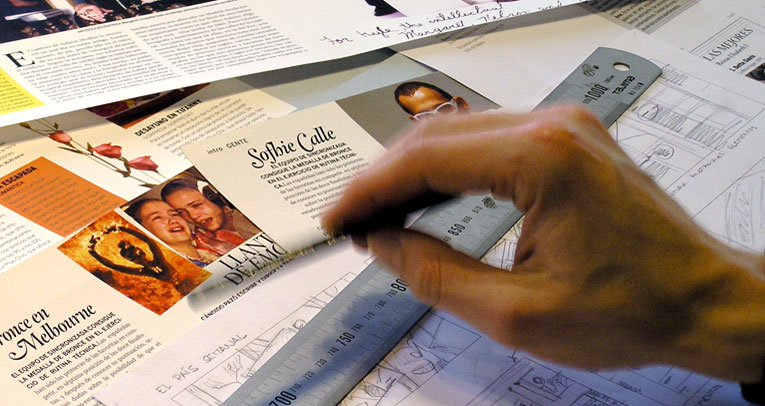
\includegraphics[scale=.08]{images/maquetador}
                    \caption{El maquetador}
                \end{subfigure}

                \vspace*{.25cm}				

                \begin{subfigure}[b]{0.5\textwidth} 
                    \centering
                    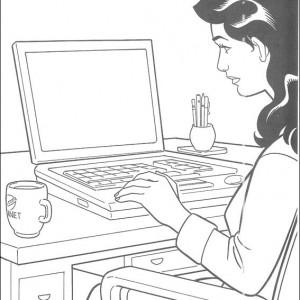
\includegraphics[scale=.12]{images/compositor}
                    \caption{El compositor}
                \end{subfigure}
            \end{figure}	
            \newpage

            \vspace*{.50cm}
            $\rightarrow$ env\'ia su manuscrito a la editorial (al maquetador). 

            \vspace*{.70cm}
            $\rightarrow$ recibe el manuscrito del autor y decide el aspecto del documento y env\'ia instrucciones al compositor.

            \vspace*{.50cm}
            $\rightarrow$ recibe las instrucciones del maquetador y compone el libro en base a tales instrucciones.
        \end{multicols}
    \end{block}
\end{frame}
%%%%%%%%%%%%%%%%

%Producción de textos estructurados con LaTeX
\begin{frame}{Generalidades}
    \begin{block}{Producci\'on de textos estructurados en \LaTeX{}.}
        \vspace{-.4cm}
        \begin{multicols}{2}
            \begin{figure}
                \centering
                \begin{subfigure}[b]{0.5\textwidth} 
                    \centering
                    
\includegraphics[scale=.08]{images/autor_LaTeX}
                    \caption{El autor}			
                \end{subfigure}

                \vspace*{.25cm}			

                \begin{subfigure}[b]{0.5\textwidth} 
                    \centering
                    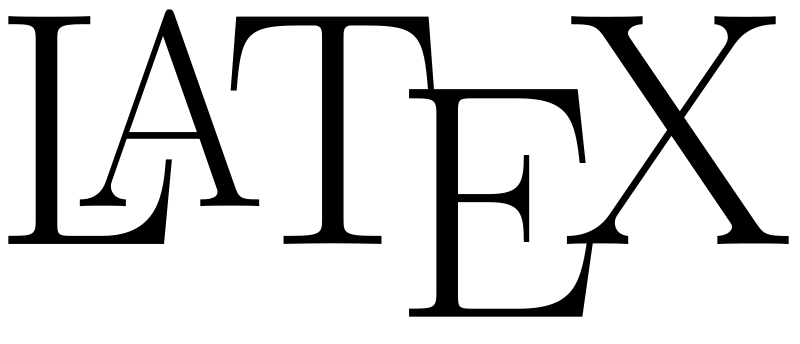
\includegraphics[scale=.09]{images/maquetador_LaTeX}
                    \caption{El maquetador}
                \end{subfigure}

                \vspace*{.25cm}				

                \begin{subfigure}[b]{0.5\textwidth} 
                    \centering
                    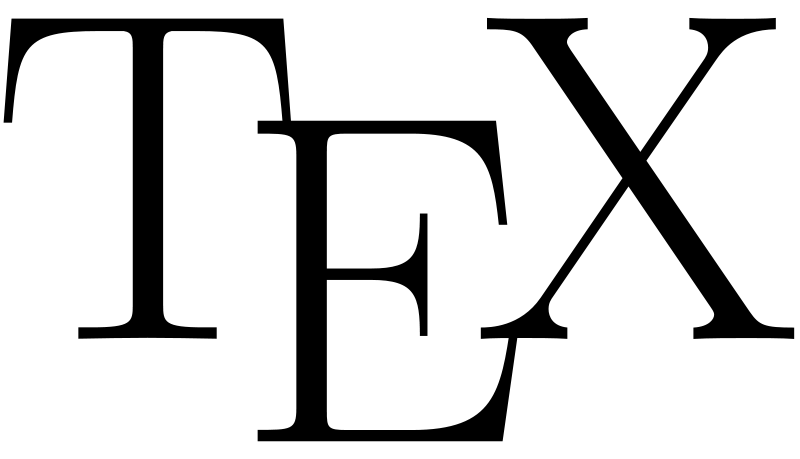
\includegraphics[scale=.06]{images/compositor_LaTeX}
                    \caption{El compositor}
                \end{subfigure}
            \end{figure}	
            \newpage

            \vspace*{.05cm}
            $\rightarrow$ Escribe el texto y \textbf{proporciona informaci\'on para describir la estructura l\'ogica de su trabajo}.


            \vspace*{.70cm}
            $\rightarrow$ interpreta la informaci\'on proveída por el autor y env\'ia las directrices al compositor.

            \vspace*{.90cm}
            $\rightarrow$ recibe las instrucciones de \LaTeX{} y compone el libro.
        \end{multicols}
    \end{block}
\end{frame}
%%%%%%%%%%%%%%%%


\begin{frame}{Generalidades}
    \begin{block}{\LaTeX{} vs MS Word}
        \begin{figure}
            \centering
            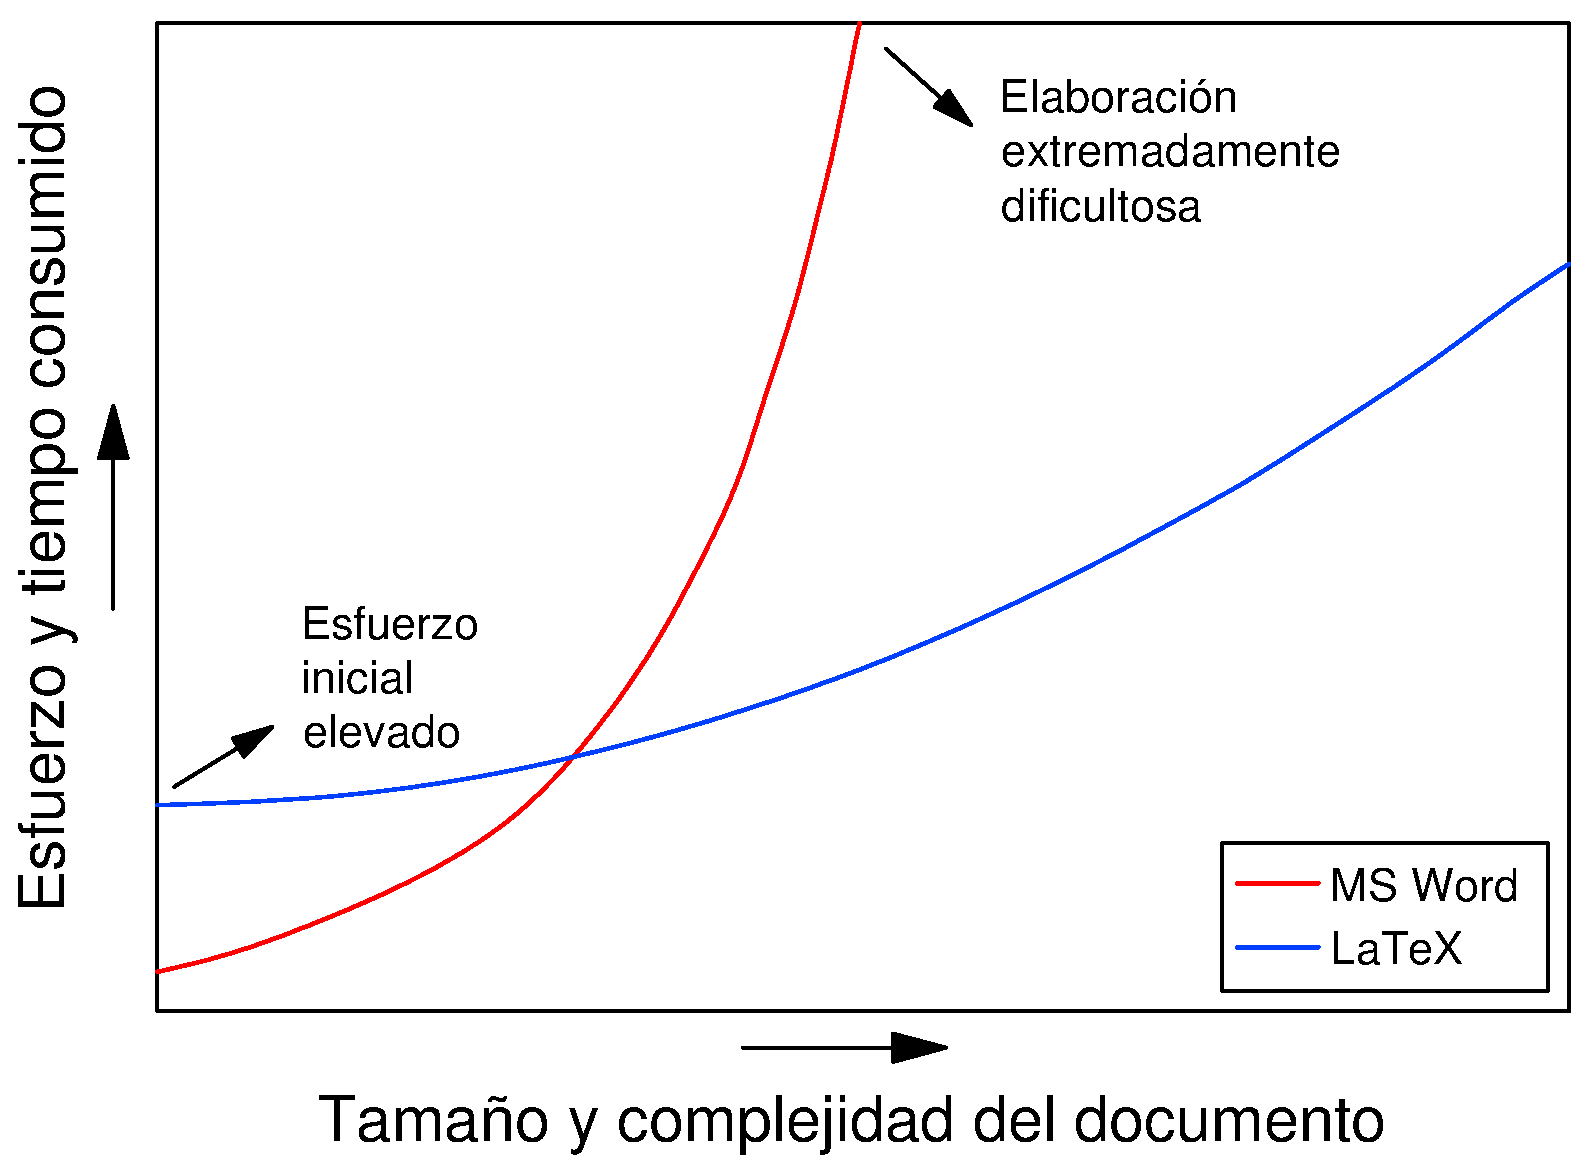
\includegraphics[scale=.3]{images/LaTeX_vs_Word.pdf}
        \end{figure}
        \begin{center}
            Si es dif\'icil de aprender vale la pena.
        \end{center}
    \end{block}
\end{frame}
%%%%%%%%%%%%%%%%

\section{Probando...}
\begin{frame}{Probando el funcionamiento}
    \begin{block}{Serie de instrucciones}
        \textbackslash documentclass[10pt,a4paper]\{article\} \\
        \textbackslash usepackage[utf8]\{inputenc\} \\
        \textbackslash begin\{document\} \\
        \textbackslash section\{Hola Mundo!\} \\
        Bienvenido al mundo de \textbackslash LaTeX \\
        \textbackslash end\{document\}
    \end{block}
\end{frame}

%%%%%%%%%%%%%%%%

\section{Archivos de entrada \LaTeX{}}

\begin{frame}{Archivos de entrada}
    \begin{itemize}
        \item \emph{Varios caracteres consecutivos} en blanco se tratan como un \emph{solo} ``espacio''. 
        \item Espacios en blanco al principio de una l\'inea se ignoran y un salto de l\'inea aislado se trata como ``espacio''
    \end{itemize}
    \begin{exampleblock}{Ejercicio 01}
        Escribir la palabra ``Hola'' seguida de 10 espacios blancos y luego ``Mundo''.
    \end{exampleblock}
    \begin{exampleblock}{Ejercicio 02}
        Escribir la palabra ``Hola'' seguida de 10 quiebres de linea (la tecla Enter) y luego ``Mundo''.
    \end{exampleblock}
\end{frame}
%%%%%%%%%%%%%%%%

\begin{frame}{Archivos de entrada \LaTeX{}}
    Son s\'imbolos reservados:
    \begin{itemize}
        \item \# \hspace*{1em} \$ \hspace*{1em} \% \hspace*{1em} \^{} \hspace*{1em} \& \hspace*{1em} \_ \hspace*{1em} \{ \hspace*{1em} \} \hspace*{1em} \~{} \hspace*{1em} $\backslash$
        \item Para que \LaTeX{} imprima estos s\'imbolos debemos escribir: \\
            $\backslash$\# \hspace*{.7em} $\backslash$\$ \hspace*{.7em} $\backslash$\% \hspace*{.7em} $\backslash$\^{}\{\} \hspace*{.7em} $\backslash$\& \hspace*{.7em} $\backslash$\_ \hspace*{.7em} $\backslash$\{ \hspace*{.7em} $\backslash$\} \hspace*{.7em} $\backslash$\~{}\{\} \hspace*{.7em} \$$\backslash$backslash\$
        \item Para imprimir acentos: \\ seguidos del tipo de acento (' o \textasciitilde). 
    \end{itemize}
    \begin{exampleblock}{Ejercicio 03}
    Generar correctamente la siguiente salida en \LaTeX{}: \\ \# $\backslash$ \$ \& $\backslash$ 	\} \{
    \end{exampleblock}
\end{frame}
%%%%%%%%%%%%%%%

\begin{frame}{Archivos de entrada \LaTeX{}}
    \begin{block}{Ordenes \LaTeX{}}
        Las \'ordenes \LaTeX{} son sensibles a may\'usculas, y adoptan uno de los formatos siguientes:
        \begin{itemize}
            \item Comienzan con una barra invertida $\backslash$ y luego tienen un nombre que consiste sólo en letras. 
                Los nombres de orden terminan con un espacio
            \item Consisten en una barra invertida y exactamente una no letra.
        \end{itemize}	
    \end{block}

    \begin{exampleblock}{Ejercicio 04}
        Probar que $\backslash$TeX $\backslash$LaTeX produce lo mismo que $\backslash$TeX$\backslash$LaTeX
    \end{exampleblock}	
    %	\begin{exampleblock}{Ejercicio 05}
    %		Probar que $\backslash$\# $\backslash$\$ \textbf{NO} produce lo mismo que $\backslash$\#$\backslash$\$
    %	\end{exampleblock}
\end{frame}
%%%%%%%%%%%%%%%%%

\begin{frame}{Archivos de entrada \LaTeX{}}
    \begin{block}{Comentarios}
        Cuando \LaTeX{} encuentra un caracter \% prescinde el resto de la l\'inea actual, 
        el salto de l\'inea y todo el espacio en blanco al comienzo de la l\'inea siguiente.
    \end{block}
    \begin{exampleblock}{Ejercicio 05}
        Probar:\\
        Este es un \% est\'upido \\
        \% REALMENTE ESTÚPIDO \\
        \hspace{2cm} ejemplo de c\'omo se puede usar el \% \\
        \hspace{1cm} s\'imbolo de comentario.
    \end{exampleblock}
\end{frame}
%%%%%%%%%%%%%%%%

\section{Estructura del archivo de entrada}

\begin{frame}{Estructura del fichero de entrada}
    \begin{block}{Partes del fichero de entrada}
        \textbf{TODO} documento escrito en \LaTeX{} consta de dos partes: \textbf{el pr\'eambulo} y el \textbf{cuerpo del texto}.
        \begin{itemize}
            \item El pr\'eambulo \textbf{siempre} empieza por la orden \\
                \texttt{$\backslash$documentclass\{...\}} \\
                Esto indica que tipo de documento se pretende escribir. 
                Luego de definir el tipo de documento se establecen los paquetes a utilizar \\
                \texttt{$\backslash$usepackage\{...\}}
            \item El cuerpo del texto comienza con la orden
                \texttt{$\backslash$begin\{document\}} \\
                Al final del documento \\
                \texttt{$\backslash$end\{document\}}\\
                Cualquier cosa que preceda esta última orden será ignorada por \LaTeX{}.
        \end{itemize}
    \end{block}
\end{frame}

\begin{frame}
    \begin{block}{Serie de instrucciones}
        \textbackslash documentclass[10pt,a4paper]\{article\} \\
        \textbackslash usepackage[utf8]\{inputenc\} \\
        \textbackslash begin\{document\} \\
        \textbackslash Hola Mundo!\\
        Bienvenido al mundo de \textbackslash LaTeX \\
        \textbackslash end\{document\}
    \end{block}
\end{frame}
%%%%%%%%%%%%%%%%

\section{El aspecto del documento}

\begin{frame}{El aspecto del documento}
\begin{block}{Clases de documento}
Esto se indica con la orden \texttt{$\backslash$documentclass}.\\
\texttt{$\backslash$documentclass[opciones]\{clase\}} \\
\emph{clase} indica el tipo de documento, con \emph{opciones} para personalizar.
    \end{block}

    \begin{exampleblock}{Ejemplo 01}
        Un archivo de entrada para un documento \LaTeX{} podría empezar con la l\'inea\\
        \texttt{$\backslash$documentclass[11pt,twoside,a4paper]\{article\}}
    \end{exampleblock}			
\end{frame}
%%%%%%%%%%%%%%%

\begin{frame}{Clases de documentos}
\begin{itemize}
    \item \texttt{article}, \texttt{minimal}, \texttt{report}, \pause
    \item \texttt{beamer:} para la producción de diapositivas \textbf{(Esta clase se utiliz\'o para preparar estos slides.)}
\end{itemize}
\end{frame}
%%%%%%%%%%%%%%%

\begin{frame}{Opciones de clases de documentos}
Hay muchas opciones.
\begin{itemize}
    \item Tama\~no de letra \item \texttt{10pt, 11pt, 12pt} \pause
    \item Tama\~no de papel \item \texttt{a4paper, letterpaper,...} \pause
    \item $\ldots$
\end{itemize}
\end{frame}
%%%%%%%%%%%%%%%

\begin{frame}{Paquetes}
    Los paquetes se incluyen. Son librer\'ias de c\'odigo \TeX\\
    \texttt{$\backslash$usepackage[opciones]\{paquete\}}\\

    \begin{alertblock}{Información sobre paquetes}
        Si tienen alguna duda sobre un paquete: Nombre del Paquete + "latex" en google.
    \end{alertblock}
\end{frame}
%%%%%%%%%%%%%%%

\begin{frame}{Estilos de p\'agina}
    \begin{block}{Tipos de estilo}
        \LaTeX{} soporta tres combinaciones predifinidas de cabeceras y pies de página, llamadas estilos de p\'agina. \\
        \texttt{$\backslash$pagestyle\{estilo\}} \\
        Los estilos son:
        \begin{itemize}
            \item \texttt{plain} imprime los n\'umeros de página en la parte de abajo, en el centro del pie. 
            \item \texttt{headings} imprime el nombre del capítulo actual y el n\'umero de p\'agina en la cabecera de cada p\'agina, mientras que el pie queda vac\'io.
            \item \texttt{empty} sin cabecera ni pie de p\'agina.
        \end{itemize}
        Para cambiar el estilo: \\
        \texttt{$\backslash$thispagestyle\{estilo\}}
    \end{block}
\end{frame}
%%%%%%%%%%%%%%%

\section{Proyectos grandes}

\begin{frame}{Proyectos grandes}
    Cuando se trabaja en proyectos grandes, dividir el archivo en partes.
    \texttt{$\backslash$include\{nombre-de-fichero\}}\\
    \texttt{$\backslash$include} agrega una nueva l\'inea.\\
    Para evitar esta nueva l\'inea:\\
    \texttt{$\backslash$input\{nombre-de-fichero\}}
\end{frame}
%%%%%%%%%%%%%%%

\section{Usemos \LaTeX}

\begin{frame}{Ejercicio 06}
    Copiar dos cap\'itulo del Tao of programming (disponible en el classroom) con el formato siguiente:
\end{frame}
%%%%%%%%%%%%%%%

\begin{frame}{Ejercicio 06}
    \begin{exampleblock}{Especificaciones requeridas}
        \begin{itemize}
            \item Clase de documento: art\'iculo
            \item Opciones de clases de documento: 
                \begin{itemize}
                    \item Letra 11pt
                    \item Papel A4
                    \item A dos columnas
                \end{itemize}
        \end{itemize}
    \end{exampleblock}

\end{frame}
%%%%%%%%%%%%%%%

\begin{frame}{Ejercicio 06}
    \begin{exampleblock}{Consideraciones importantes}
        \begin{itemize}
            \item Para crear el título del documento utiliza la orden \texttt{$\backslash$title\{t\'itulo\}} y en el pre\'ambulo.
                Luego escribe la orden \texttt{$\backslash$maketitle} al incio del cuerpo del texto.
            \item Para crear un resumen:\\
                \texttt{$\backslash$begin\{abstract\}} \\
                \textit{Escribir el resumen} \\
                \texttt{$\backslash$end\{abstract\}}
            \item Para crear una secci\'on usa la orden \texttt{$\backslash$section\{...\}}
            \item Para crear una subsecci\'on usa la orden \texttt{$\backslash$subsection\{...\}}
        \end{itemize}
    \end{exampleblock}
\end{frame}
%%%%%%%%%%%%%%%

\section{Saltos de l\'inea y p\'agina}

\begin{frame}{Saltos de l\'inea y de p\'agina}
    \begin{block}{Justificaci\'on de p\'arrafos}
        \begin{itemize}
            \item Salte de l\'inea con: \texttt{$\backslash\backslash$} o \texttt{$\backslash$newline}
            \item Salto forzado de página: \texttt{$\backslash$newpage}
            \item La orden: \texttt{$\backslash\backslash$*} \\ prohibe que exista un salto de p\'agina tras el salto forzado de l\'inea.
        \end{itemize}
    \end{block}
\end{frame}
%%%%%%%%%%%%%%%

\begin{frame}{Saltos de l\'inea y de p\'agina}
    \begin{block}{Evitar separaciones}
        \begin{itemize}
            \item A veces es necesario mantener un argumento sin que se separe.  \texttt{$\backslash$mbox\{...\}} 
        \end{itemize}
    \end{block}
\end{frame}
%%%%%%%%%%%%%%%

\begin{frame}{Saltos de l\'inea y de p\'agina}
    \begin{exampleblock}{Ejercicio 07}
        \begin{itemize}
            \item Genera la siguiente salida: \\
                Este es un ejemplo \\
                de c\'omo \newline
                realizar saltos de \\
                l\'inea.
            \item Genera la siguiente salida: \\
                \fbox{Este es un ejemplo del uso de $\backslash$fbox}
            \item Genera la siguiente salida sin que se silabe el n\'umero de cuenta:\\
                El n\'umero de cuenta en la que debes realizar el dep\'osito es 123 456 789 555 000, puedes pasar esta tarde por el banco.
        \end{itemize}
    \end{exampleblock}
\end{frame}
%%%%%%%%%%%%%%%

\section{S\'imbolos}

    \begin{frame}{Comillas}
        Para generar comillas no se debe usar \textbf{"}. En tipograf\'ia hay comillas especiales de apertura y cierre.\\
        En \LaTeX{}, se utilizan dos acentos graves para abrir comillas y dos ap\'ostrofes para cerrar comillas. \\
        Para comillas simples basta con un ap\'ostrofe.

        \begin{exampleblock}{Ejercicio 08}
            \begin{itemize}
                \item Genere las siguientes salidas: \\
                    ``Este es un ejemplo del correcto uso de comillas'' \\
                    \fbox{Estoy aprendiendo a usar ``\LaTeX{}''. ¡Odio este tema!}\\
                    Ahora ya aprend\'i que el comando \fbox{``\%''} se utiliza para hacer 'comentarios'. 	
             \end{itemize}
        \end{exampleblock}
    \end{frame}
    %%%%%%%%%%%%%%%

    \begin{frame}{Guiones y rayas}
        En \LaTeX{} existen cuatro tipos distintos de gui\'on:

        \begin{block}{¿Cómo obtenerlos?}
            \begin{itemize}
                \item Guión ``-''
                \item Raya corta ``--''
                \item Raya ``---''
            \end{itemize}

        \end{block}
        El resto de los s\'imbolos? Mirar el archivo LatexSimbols.pdf en el classroom.
    \end{frame}
    %%%%%%%%%%%%%%%
    %%%%%%%%%%%%%%%

    \section{T\'itulos, cap\'itulos y secciones}

    \begin{frame}{T\'itulos, cap\'itulos y secciones}

        Las siguientes \'ordenes estan disponibles para la clase \texttt{article}: \\
        \begin{itemize}
            \item \texttt{$\backslash$section\{...\}} \\
            \item \texttt{$\backslash$subsection\{...\}} \\
            \item \texttt{$\backslash$subsubsection\{...\}} \\
            \item \texttt{$\backslash$paragraph\{...\}} \\
            \item \texttt{$\backslash$subparagraph\{...\}}
        \end{itemize}
        Si se quiere dividir el documento en partes sin influir la numeraci\'on de secciones o capítulos se puede usar:
        \begin{itemize}
            \item \texttt{$\backslash$part\{...\}}
        \end{itemize}
    \end{frame}
    %%%%%%%%%%%%%%%

    \begin{frame}
        \frametitle{Indices}
        Para crear un \'indice:
        \begin{itemize}
            \item \texttt{$\backslash$tableofcontents}
        \end{itemize}
        y ubica el índice general en el lugar donde se ejecuta la orden.

        \begin{alertblock}{¡Ojo!}
            Todas las comandos de secci\'on tienen una versi\'on ``estrella'' seguidas de un asterisco (\texttt{$\backslash$section\{...\}*}).
                Generan encabezados de secci\'on pero no aparecen en el \'indice y no se enumeran.
        \end{alertblock}

        \begin{alertblock}{Títulos muy largos}
            Si un encabezado es muy largo:
            \texttt{$\backslash$section[T\'itulo para el \'indice general]\{Un largo y aburrido t\'itulo que va a a aparecer en el texto. \}}
        \end{alertblock}

    \end{frame}
    %%%%%%%%%%%%

    \begin{frame}
        \begin{block}{T\'itulo general}
            El t\'itulo de todo el documento se genera:
            \begin{itemize}
                \item  \texttt{$\backslash$maketitle}
            \end{itemize}
            El contenido del t\'itulo tiene que definirse en el pre\'ambulo:
            \begin{itemize}
                \item \texttt{$\backslash$title\{...\}}
                \item \texttt{$\backslash$author\{...\}}
                \item \texttt{$\backslash$date\{...\}}
            \end{itemize}

            En el argumento \texttt{$\backslash$author} se pueden poner varios nombres separado por \texttt{$\backslash$and}
        \end{block}

        \begin{exampleblock}{Ejercicio 10}
            \begin{itemize}
                \item Generar el \'indice general y completar los datos de autor y fecha para el texto del Ejercicio 06.
            \end{itemize}
        \end{exampleblock}
    \end{frame}
    %%%%%%%%%%%%%%%

    \section{Notas al pie}

    \begin{frame}{Notas al pie}
        Con la orden \\
        \texttt{$\backslash$footnote\{\emph{texto al pie}\}} \\
        se imprime una nota al pie en la p\'agina actual. 
            
        \begin{exampleblock}{Ejercicio 11}
            \begin{itemize}
                \item Escriba una nota al pie en el texto del Ejercicio 06 para comprobar su funcionamiento.
            \end{itemize}
        \end{exampleblock}

    \end{frame}

    \section{Estilos de letra}

    \begin{frame}{Estilos de letra}
        \begin{block}{Los distintos estilos}
            \LaTeX{} tiene varios estilos de letra que pueden ser utilizados, ellos son: \\
            \begin{itemize}
                \item \textbf{Negrita} \texttt{$\backslash$textbf\{...\}}
                \item \textit{Cursiva} \texttt{$\backslash$textit\{...\}}
                \item \texttt{M\'aquina de escribir} \texttt{$\backslash$texttt\{...\}}
                \item \emph{Enfasis} \texttt{$\backslash$emph\{...\}}
            \end{itemize}
        \end{block}

        \begin{exampleblock}{Ejercicio 12}
            \begin{itemize}
                \item Genere la siguiente salida. \\
                    Yo estudio \textbf{Ingenier\'ia Industrial} \textit{estar\'ia bueno saber} en que ``met\'i''. \\
            \end{itemize}
        \end{exampleblock}
    \end{frame}
